\documentclass[11pt]{article}
\usepackage[margin=1in]{geometry}
\usepackage{mathptmx}
\usepackage[T1]{fontenc}
\usepackage{booktabs}
\usepackage{graphicx}
\usepackage{caption}
\usepackage{amsmath}
\usepackage[hidelinks]{hyperref}
\captionsetup{font=small}
\setlength{\parskip}{3pt}
\title{Classifying Query--Product Relevance on Amazon ESCI with Lexical Baselines, Cross-Encoders and a Stacked Hybrid\\[4pt]\large CMPS261 Final Project Report (Option 4.2)}
\author{Allie Saoud \and Zulfiquar Fneiche}
\date{}
\begin{document}
\maketitle

\begin{abstract}
We classify shopping query--product pairs from the Amazon Shopping Queries dataset (ESCI) into Exact, Substitute, Complement and Irrelevant.
On the US reduced set (601{,}354 pairs) we compare a majority-class baseline, logistic regression on TF-IDF, LightGBM on 33 hand-built lexical features, three fine-tuned pretrained cross-encoders (MiniLM-L6, DeBERTa-v3-small and DeBERTa-v3-base) and a LightGBM stacker that combines cross-encoder probabilities with the lexical features.
All model choices were made on a validation split grouped by query, and the held-out test split was evaluated once.
The selected model, DeBERTa-v3-base, reaches test micro-F1 0.608 and macro-F1 0.555, against 0.527 and 0.393 for LightGBM.
The Complement class stays hardest (test F1 0.446), and 52.3\% of the remaining errors are confusions between Exact and Substitute.
We also report ablations on product fields, sequence length, class weighting, training-set size and random seed, and the compute cost of each model.
\end{abstract}

\section{Introduction}
When a customer searches an online store, the store has to decide how well each product matches the query.
The ESCI dataset \cite{reddy2022} labels this with four classes: \emph{Exact} (the product is what was asked for), \emph{Substitute} (it is close and could replace it), \emph{Complement} (it goes with the requested product) and \emph{Irrelevant}.
The task is hard because the classes depend on small details: for a query ``phone case for iPhone 12'', an iPhone 12 would be a Complement and a case for an iPhone 11 a Substitute or Irrelevant.
Word overlap alone does not separate these cases.

Our questions were: (1) how far a well-tuned lexical model gets, (2) how much pretrained cross-encoders add, and which design choices matter for them, and (3) whether combining both helps.
Our progress report covered the baselines and two cross-encoders. This report adds a larger cross-encoder, a set of controlled ablations, the hybrid stacker, a resource analysis and the one-time test evaluation.
All code, the notebook, run logs and the trained models are in our repository: \url{https://github.com/CakeLiar/cmps261-esci}.

\section{Dataset}
We use the US locale of the reduced version (\texttt{small\_version == 1}) of the ESCI data \cite{reddy2022}, joined with the product catalogue (482{,}105 products).
No pairs had a missing product and there were no duplicate pairs.
Product titles are always present, but descriptions are missing for 47.8\% of products, bullet points for 13.2\%, brand for 5.6\% and colour for 32.2\%.
Queries are short (mean 4.0 words) and titles are long (mean 17.1 words).

\textbf{Cleaning.} We unescape HTML, strip tags, normalise whitespace and lowercase all text. Missing fields become empty strings.

\textbf{Splits.} We keep the official test split untouched. From the official training split we hold out 10\% of \emph{queries} (not pairs) as validation, with seed 42, so that no query appears in both training and validation.
Table~\ref{tab:data} shows the sizes and label shares. The classes are imbalanced: Complement is under 5\% of pairs.

\begin{table}[h]\centering\small
\begin{tabular}{lrrrrrr}\toprule
Split & Queries & Pairs & E & S & C & I \\\midrule
Train & 18{,}800 & 377{,}484 & 43.3\% & 35.2\% & 4.6\% & 17.0\% \\
Validation & 2{,}088 & 42{,}169 & 43.9\% & 34.9\% & 4.4\% & 16.8\% \\
Test & 8{,}956 & 181{,}701 & 43.9\% & 35.0\% & 4.5\% & 16.7\% \\
\bottomrule\end{tabular}
\caption{Split sizes and label distribution.}\label{tab:data}
\end{table}

\textbf{Metric.} Following the KDD Cup 2022 task 2 \cite{reddy2022} we use micro-F1 (equal to accuracy for single-label classification) as the main metric, and also report macro-F1 and per-class F1, because micro-F1 hides poor performance on Complement.

\section{Models}
\textbf{Majority class.} Always predicts Exact.

\textbf{Lexical features + LightGBM.} We compute 33 features per pair: token and character overlap between the query and the title, bullets, brand and colour; BM25-style scores \cite{robertson2009}; query and title lengths; whether the query contains numbers, units or negations; and whether query numbers appear in the title.
We train LightGBM \cite{ke2017} with learning rate 0.05 and early stopping (50 rounds) on validation, and tune \texttt{num\_leaves} $\in\{31,127\}$, \texttt{min\_child\_samples} $\in\{50,200\}$ and class weights (none or balanced): 8 settings.
The best used 127 leaves, minimum 200 samples per leaf, no class weights, and stopped at 99 trees.

\textbf{Logistic regression.} Multinomial logistic regression \cite{pedregosa2011} on word and character TF-IDF of the query and title (1{,}045{,}120 sparse columns, fit on training text only) plus the standardised lexical features, with $C\in\{0.1,0.3,1,3\}$ and optional balanced class weights.
In the progress report these fits stopped at 300 lbfgs iterations without converging. With the iteration limit raised to 3{,}000, 8 of 8 settings converged; the best (C=0.1, class weight none) reached validation micro-F1 0.520, against 0.519 at 300 iterations.

\textbf{Cross-encoders.} A cross-encoder reads the query and the product text as one sequence and classifies the pair from the joint representation \cite{nogueira2019}.
We fine-tune three pretrained encoders with a new 4-class head and cross-entropy loss: MiniLM-L6 \cite{wang2020}, already trained as a passage re-ranker on MS MARCO \cite{bajaj2016}; DeBERTa-v3-small and DeBERTa-v3-base \cite{he2023}.
Input A is the cleaned query; input B is the title, brand and colour, and the first 300 characters of the bullet points, joined with the separator token and truncated to 128 tokens.
We train for 2 epochs with AdamW \cite{loshchilov2019} (weight decay 0.01, 5\% linear warm-up, then linear decay), learning rate $3\times10^{-5}$ and batch 64 for MiniLM and $2\times10^{-5}$ and batch 48 for DeBERTa, with mixed precision \cite{wolf2020}.
We evaluate on validation every 2,000 steps and keep the checkpoint with the best micro-F1.

\textbf{Hybrid stacker.} Cross-encoders read text but cannot see our hand-built signals directly (for example, whether a number in the query is in the title), and LightGBM cannot read text. We therefore stack them \cite{wolpert1992}: a second LightGBM takes the cross-encoders' class probabilities and the 33 lexical features.
Because the cross-encoders were trained on the training split, their probabilities on training pairs are over-confident. We train the stacker on the \emph{validation} split instead and score it with 5-fold cross-validation grouped by query, so every validation prediction comes from a model that did not see that query.
We compared four inputs (Table~\ref{tab:hybrid}) with fixed settings (300 trees, learning rate 0.05, 31 leaves, minimum 100 samples per leaf) and chose by out-of-fold micro-F1.

\textbf{Model selection.} The final model is the one with the highest validation micro-F1 (out-of-fold for the stacker). For the test run, the selected stacker is refit on all validation pairs.

\section{Results}
All training ran on Google Cloud VMs with one NVIDIA L4 GPU (24\,GB) and 32 vCPUs each.

\subsection{Validation results and model selection}
\begin{table}[h]\centering\small
\begin{tabular}{lrrrrrr}\toprule
Model & micro-F1 & macro-F1 & F1 E & F1 S & F1 C & F1 I \\\midrule
Majority class (always E) & 0.439 & 0.152 & 0.610 & 0.000 & 0.000 & 0.000 \\
Logistic regression (TF-IDF + features) & 0.520 & 0.383 & 0.610 & 0.494 & 0.095 & 0.334 \\
LightGBM (33 lexical features) & 0.524 & 0.396 & 0.612 & 0.502 & 0.115 & 0.353 \\
MiniLM-L6 & 0.582 & 0.510 & 0.666 & 0.532 & 0.381 & 0.462 \\
DeBERTa-v3-small & 0.599 & 0.548 & 0.661 & 0.584 & 0.450 & 0.500 \\
DeBERTa-v3-base & 0.612 & 0.562 & 0.677 & 0.580 & 0.453 & 0.537 \\
Hybrid stacker, lexical + all cross-encoders (5-fold OOF) & 0.607 & 0.549 & 0.675 & 0.577 & 0.420 & 0.524 \\
\bottomrule\end{tabular}
\caption{Validation results (42{,}169 pairs). Cross-encoders: best checkpoint. Stacker: 5-fold out-of-fold predictions.}\label{tab:val}
\end{table}

Table~\ref{tab:val} shows the main comparison. LightGBM improves on the majority baseline mostly on Substitute and Irrelevant but almost never predicts Complement (F1 0.115).
Every cross-encoder beats it, with the largest gains on Complement and Irrelevant. Larger encoders do better: MiniLM-L6 0.582, DeBERTa-v3-small 0.599, DeBERTa-v3-base 0.612 micro-F1.

\subsection{Hybrid stacker}
\begin{table}[h]\centering\small
\begin{tabular}{lrrrrrr}\toprule
Input & micro-F1 & macro-F1 & F1 E & F1 S & F1 C & F1 I \\\midrule
MiniLM-L6 alone & 0.582 & 0.510 & 0.666 & 0.532 & 0.381 & 0.462 \\
DeBERTa-v3-small alone & 0.599 & 0.548 & 0.661 & 0.584 & 0.450 & 0.500 \\
DeBERTa-v3-base alone & 0.612 & 0.562 & 0.677 & 0.580 & 0.453 & 0.537 \\
Stacker: cross-encoder probabilities only & 0.607 & 0.550 & 0.673 & 0.574 & 0.425 & 0.528 \\
Stacker: lexical + best cross-encoder & 0.603 & 0.544 & 0.671 & 0.574 & 0.419 & 0.513 \\
\textbf{Stacker: lexical + all cross-encoders} & \textbf{0.607} & \textbf{0.549} & \textbf{0.675} & \textbf{0.577} & \textbf{0.420} & \textbf{0.524} \\
Stacker: lexical + all cross-encoders, balanced & 0.584 & 0.541 & 0.642 & 0.574 & 0.420 & 0.529 \\
\bottomrule\end{tabular}
\caption{Hybrid stacker variants, validation, 5-fold out-of-fold grouped by query. ``Alone'' rows are the cross-encoders' own argmax on the same pairs.}\label{tab:hybrid}
\end{table}

The best input is lexical + all cross-encoders (Table~\ref{tab:hybrid}). Compared with the best single cross-encoder, DeBERTa-v3-base, on the same pairs it changes micro-F1 by -0.004 and macro-F1 by -0.013.
So stacking did not help: the stacker is trained on validation pairs only (about four fifths of 42{,}169 per fold), and the lexical features add little that the cross-encoders do not already capture. Adding the lexical features to the best cross-encoder alone (0.603) also scores below that cross-encoder by itself.
Balanced class weights in the stacker lower micro-F1 to 0.584 and leave Complement F1 unchanged (0.420 against 0.420).

\subsection{Ablations (MiniLM-L6, validation)}
To find which design choices matter we changed one setting at a time on MiniLM-L6, the cheapest cross-encoder (Table~\ref{tab:abl}).

\begin{table}[h]\centering\small
\begin{tabular}{lrrrrr}\toprule
Setting & micro-F1 & macro-F1 & F1 C & F1 I & Train min \\\midrule
Reference: title, brand+colour, bullets; length 128 & 0.582 & 0.510 & 0.381 & 0.462 & 11.7 \\
Title only & 0.572 & 0.496 & 0.357 & 0.443 & 8.7 \\
Title + bullets & 0.579 & 0.509 & 0.386 & 0.462 & 8.7 \\
Reference fields + description & 0.582 & 0.528 & 0.408 & 0.496 & 8.7 \\
Max length 64 & 0.578 & 0.517 & 0.391 & 0.469 & 6.4 \\
Max length 256 & 0.581 & 0.526 & 0.409 & 0.484 & 18.4 \\
Class-weighted loss (balanced) & 0.531 & 0.491 & 0.349 & 0.487 & 8.7 \\
Seed 1 instead of 0 & 0.586 & 0.529 & 0.411 & 0.492 & 8.7 \\
\bottomrule\end{tabular}
\caption{One-change-at-a-time ablations on MiniLM-L6 (best validation checkpoint). The reference run is from the first round, on a different L4 VM, so its training time is not directly comparable.}\label{tab:abl}
\end{table}

\textbf{Seed variance.} MiniLM-L6: micro-F1 0.582 (seed 0) and 0.586 (seed 1), a difference of 0.004; macro-F1 0.510 and 0.529. The DeBERTa-v3-small seed-1 run ended early, after its validation pass at step 2{,}000 of 15{,}730, without an error message (we found this only after the VM was deleted). At that shared checkpoint the two seeds give micro-F1 0.592 (seed 0) and 0.588 (seed 1), macro-F1 0.536 and 0.526. Differences between configurations smaller than this should not be read as real.

\subsection{Complexity and resource analysis}
\begin{table}[h]\centering\small
\begin{tabular}{lrrrrrr}\toprule
Model & Params & Max len & Batch & Train min & Peak GPU GB & Pairs/s (inference) \\\midrule
MiniLM-L6 & 23M & 128 & 64 & 12 & -- & 2{,}622 \\
DeBERTa-v3-small & 142M & 128 & 48 & 54 & -- & 874 \\
DeBERTa-v3-base & 184M & 128 & 48 & 94 & 8.9 & 484 \\
MiniLM-L6, length 64 & 23M & 64 & 64 & 6 & 0.8 & 12{,}778$^\dagger$ \\
MiniLM-L6, length 256 & 23M & 256 & 64 & 18 & 2.1 & 2{,}481$^\dagger$ \\
\bottomrule\end{tabular}
\caption{Cost of the cross-encoders on one L4 GPU. Train minutes cover 2 epochs including the periodic validation passes. Inference throughput is measured on the test split; $^\dagger$ from the validation passes. Peak memory was not logged in the first-round runs (--).}\label{tab:res}
\end{table}

Table~\ref{tab:res} shows the cost side. The cost of a cross-encoder grows with both model size and sequence length, while the classical models are far cheaper: the LightGBM refit took 9 seconds on CPU (99 trees) and predicted the 181{,}701 test pairs in 0.5 seconds, and the stacker adds only a small LightGBM on top of the cross-encoder outputs.
Each logistic-regression fit on 1{,}045{,}120 sparse columns took 13--39 minutes of CPU time per setting (8 settings run in parallel), about as long as fine-tuning MiniLM-L6 on the GPU, for much lower scores.

\begin{figure}[h]\centering
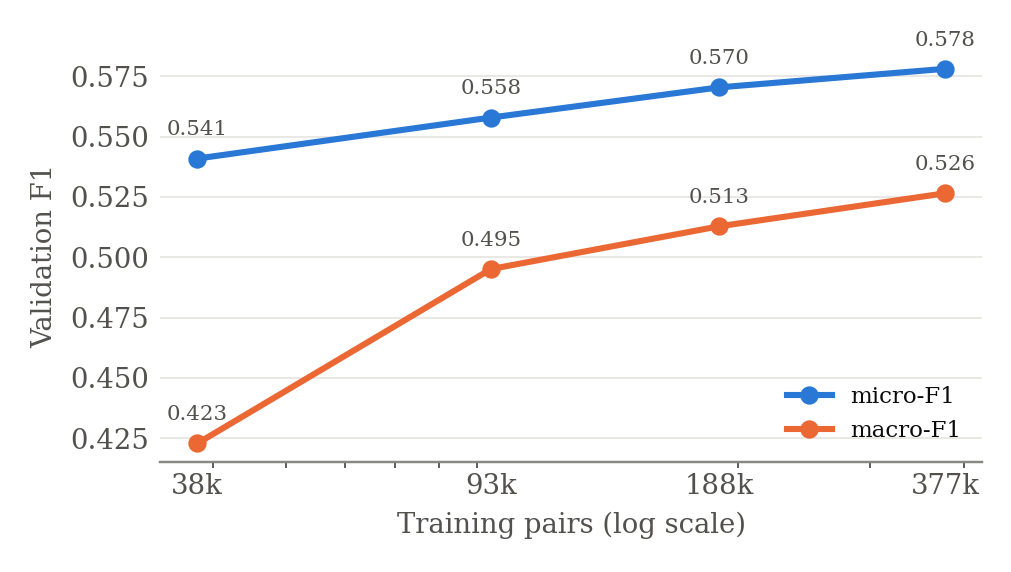
\includegraphics[width=0.62\linewidth]{../figures/final_learning_curve.png}
\caption{Learning curve for MiniLM-L6: validation F1 at the last checkpoint against the number of training pairs (training queries subsampled, seed 0).}\label{fig:curve}
\end{figure}

\begin{table}[h]\centering\small
\begin{tabular}{rrrrr}\toprule
Share of train queries & Pairs & micro-F1 & macro-F1 & F1 C \\\midrule
10\% & 38{,}118 & 0.541 & 0.423 & 0.108 \\
25\% & 93{,}813 & 0.558 & 0.495 & 0.356 \\
50\% & 188{,}735 & 0.570 & 0.513 & 0.387 \\
100\% & 377{,}484 & 0.578 & 0.526 & 0.413 \\
\bottomrule\end{tabular}
\caption{Learning curve data (MiniLM-L6, last checkpoint, validation).}\label{tab:curve}
\end{table}

Figure~\ref{fig:curve} and Table~\ref{tab:curve} show how results change with training data size.

\subsection{Test results}
\begin{table}[h]\centering\small
\begin{tabular}{lrrrrrr}\toprule
Model & micro-F1 & macro-F1 & F1 E & F1 S & F1 C & F1 I \\\midrule
Hybrid stacker (lexical + all cross-encoders) & 0.609 & 0.552 & 0.677 & 0.581 & 0.430 & 0.519 \\
\textbf{DeBERTa-v3-base $\star$} & \textbf{0.608} & \textbf{0.555} & \textbf{0.677} & \textbf{0.580} & \textbf{0.446} & \textbf{0.520} \\
DeBERTa-v3-small & 0.602 & 0.553 & 0.663 & 0.591 & 0.462 & 0.498 \\
MiniLM-L6 & 0.581 & 0.508 & 0.664 & 0.535 & 0.375 & 0.457 \\
LightGBM (lexical features) & 0.527 & 0.393 & 0.615 & 0.505 & 0.097 & 0.353 \\
Logistic regression (TF-IDF) & 0.523 & 0.384 & 0.615 & 0.495 & 0.093 & 0.335 \\
Majority class (always E) & 0.439 & 0.152 & 0.610 & 0.000 & 0.000 & 0.000 \\
\bottomrule\end{tabular}
\caption{Held-out test split (181{,}701 pairs, 8{,}956 queries), evaluated once. $\star$ marks the model chosen on validation.}\label{tab:test}
\end{table}

Table~\ref{tab:test} gives the test results. The model chosen on validation, DeBERTa-v3-base, scores 0.608 micro-F1, +0.081 over LightGBM.
Its validation micro-F1 was 0.612, so test and validation agree closely and the validation split was a reliable guide.
The hybrid stacker, which was not selected, scores 0.609 on test; the gap to the selected model is within the seed variation we measured, so we do not read it as a difference.
As a check that the saved checkpoints are the ones evaluated, re-predicting validation with each reloaded model matched the saved validation predictions on this share of pairs: MiniLM-L6 1.0000, DeBERTa-v3-small 1.0000, DeBERTa-v3-base 1.0000.

\begin{figure}[h]\centering
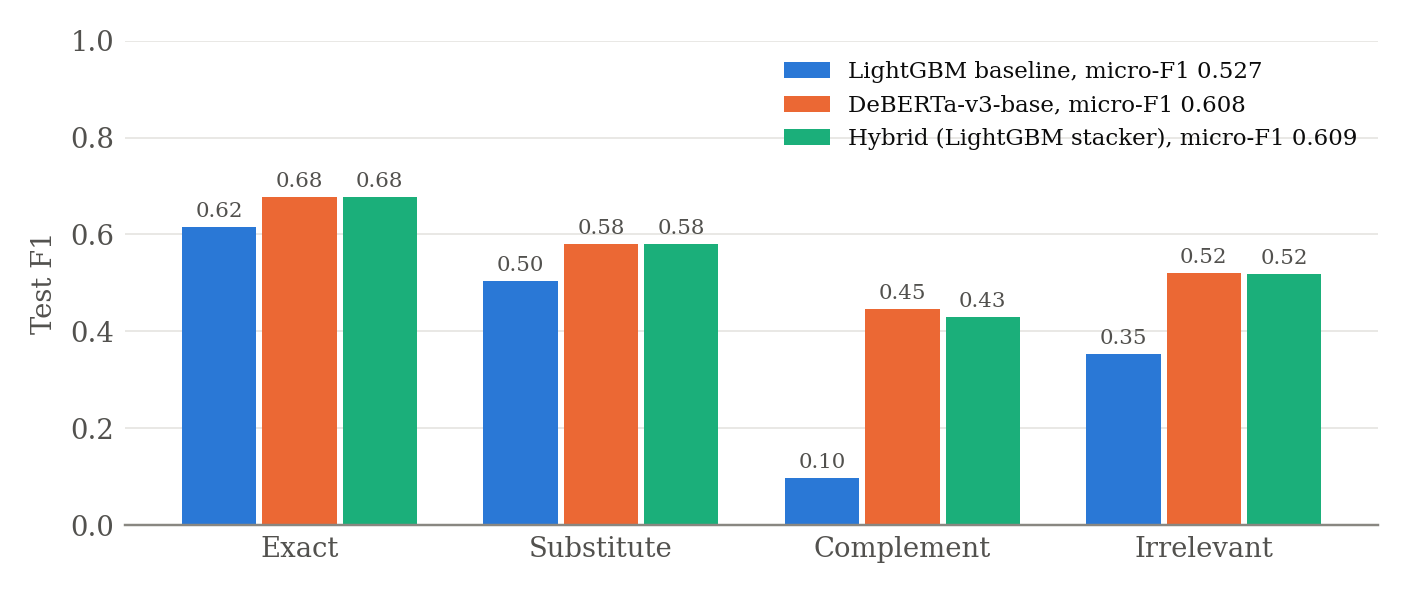
\includegraphics[width=0.85\linewidth]{../figures/final_test_per_class_f1.png}
\caption{Per-class test F1 of LightGBM, the best single cross-encoder and the hybrid stacker.}\label{fig:pc}
\end{figure}

\subsection{Failure analysis}
\begin{figure}[h]\centering
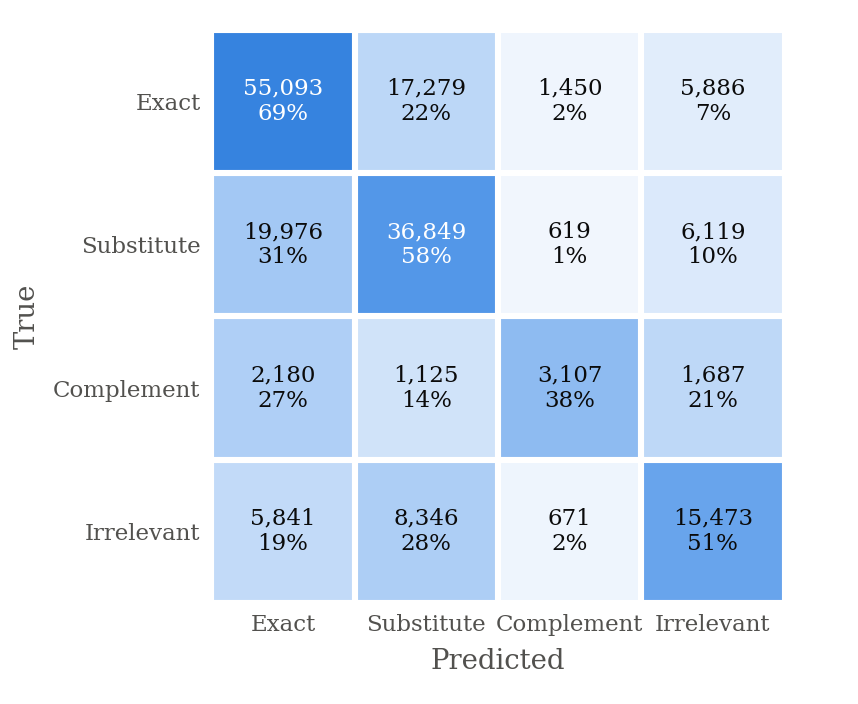
\includegraphics[width=0.48\linewidth]{../figures/final_test_confusion.png}
\caption{Test confusion matrix of the final model (row-normalised shares and counts).}\label{fig:conf}
\end{figure}

\textbf{Confusions.} In the final model's test confusion matrix (Figure~\ref{fig:conf}), 31.4\% of Substitute pairs are predicted Exact, and only 38.4\% of Complement pairs are predicted Complement (26.9\% are predicted Exact).
Exact versus Substitute often turns on a detail such as a size, model number or brand that the query names.

\textbf{Complement recall.} On validation, Complement recall is: LightGBM 6.4\%, MiniLM-L6 31.5\%, DeBERTa-v3-small 46.5\%, DeBERTa-v3-base 39.7\%.
Complement products can share many words with the query (a charger whose title names the phone the query asks for), which pushes overlap-based models towards Exact; the high-overlap slice below shows this.

\textbf{Slices.} We fixed six slices before looking at results (Table~\ref{tab:slices}): pairs with high title overlap (at least 75\% of query tokens in the title) labelled Irrelevant or Complement; pairs with low overlap (at most 25\%) labelled Exact; queries with a likely misspelling (a 4+ letter word never seen in training titles or bullets); and queries with a number or a negation.
On validation, LightGBM got only 9.0\% of the high-overlap I/C pairs right, because it relies on overlap, against 27.6\% for MiniLM-L6, 40.9\% for DeBERTa-v3-small, 39.5\% for DeBERTa-v3-base.

\begin{table}[h]\centering\small
\begin{tabular}{lrrr}\toprule
Slice & Pairs & LightGBM & DeBERTa-v3-base \\\midrule
All pairs & 181{,}701 & 0.527 & 0.608 \\
High title overlap, label I or C & 4{,}494 & 0.078 & 0.435 \\
Low title overlap, label E & 21{,}426 & 0.475 & 0.559 \\
Likely misspelled query & 16{,}618 & 0.511 & 0.565 \\
Query has a number & 37{,}584 & 0.535 & 0.635 \\
Query has a negation & 22{,}970 & 0.509 & 0.616 \\
\bottomrule\end{tabular}
\caption{Test accuracy on the failure slices.}\label{tab:slices}
\end{table}

\section{Conclusion}
Fine-tuned cross-encoders clearly beat lexical models on ESCI, mainly by recovering Complement and Irrelevant pairs that word overlap gets wrong, and larger encoders help further at a higher cost.
Stacking the cross-encoder outputs with lexical features did not beat the best single cross-encoder on validation, so our final model is DeBERTa-v3-base (test micro-F1 0.608).
The ablations show that class weighting in the loss hurts, that adding fields beyond the title helps a little, and that many differences of a few thousandths are within seed noise.
The main open problem is Complement and the Exact/Substitute boundary. Promising next steps are training on the full (not reduced) dataset, larger encoders or longer training, adding the product description through a longer input, and query-level features such as the other products retrieved for the same query.

\begin{thebibliography}{99}\small
\bibitem{reddy2022} C.~K.~Reddy et~al. Shopping Queries Dataset: A Large-Scale ESCI Benchmark for Improving Product Search. arXiv:2206.06588, 2022.
\bibitem{ke2017} G.~Ke, Q.~Meng, T.~Finley, T.~Wang, W.~Chen, W.~Ma, Q.~Ye, T.-Y.~Liu. LightGBM: A Highly Efficient Gradient Boosting Decision Tree. NeurIPS, 2017.
\bibitem{he2023} P.~He, J.~Gao, W.~Chen. DeBERTaV3: Improving DeBERTa using ELECTRA-Style Pre-Training with Gradient-Disentangled Embedding Sharing. ICLR, 2023.
\bibitem{wang2020} W.~Wang, F.~Wei, L.~Dong, H.~Bao, N.~Yang, M.~Zhou. MiniLM: Deep Self-Attention Distillation for Task-Agnostic Compression of Pre-Trained Transformers. NeurIPS, 2020.
\bibitem{nogueira2019} R.~Nogueira, K.~Cho. Passage Re-ranking with BERT. arXiv:1901.04085, 2019.
\bibitem{bajaj2016} P.~Bajaj et~al. MS MARCO: A Human Generated MAchine Reading COmprehension Dataset. arXiv:1611.09268, 2016.
\bibitem{robertson2009} S.~Robertson, H.~Zaragoza. The Probabilistic Relevance Framework: BM25 and Beyond. Foundations and Trends in Information Retrieval, 3(4), 2009.
\bibitem{loshchilov2019} I.~Loshchilov, F.~Hutter. Decoupled Weight Decay Regularization. ICLR, 2019.
\bibitem{pedregosa2011} F.~Pedregosa et~al. Scikit-learn: Machine Learning in Python. JMLR 12, 2011.
\bibitem{wolf2020} T.~Wolf et~al. Transformers: State-of-the-Art Natural Language Processing. EMNLP (System Demonstrations), 2020.
\bibitem{wolpert1992} D.~H.~Wolpert. Stacked Generalization. Neural Networks 5(2), 1992.
\end{thebibliography}
\end{document}
